\chapter{Background}
\label{background}
Deep architecture and recurrent topology have been significantly developed over the last decade that allow neural networks to automatically extract abstract and useful features. They are as of today the best tools to solve problems such as image detection \cite{krizhevsky12, girshick14}, speech recognition \cite{dahl12, deng13}, and language modelling \cite{mnih07, mikolov10}, outperforming many known machine learning models with hand-crafted feature-extractors. Since our model formulation relies mainly on deep neural networks, this chapter will begin with the basics of neural networks. 

\section{Neural networks}
Artificial neural networks are computational models that consist of interconnected adaptive units \cite{hassoun03}. A set of input is feeded to each unit, also called artificial neuron, with certain weights assigned. 

\begin{figure}
\centering
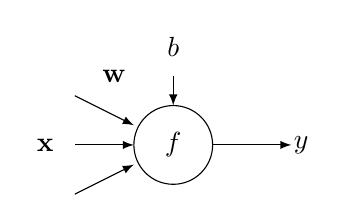
\begin{tikzpicture}[scale=2.5]
\draw (0, 0) circle (0.2cm);
\draw [-latex] (-0.5, 0.25) -- (-0.2, 0.1);
\draw [-latex] (-0.5, 0) -- (-0.2, 0);
\draw [-latex] (-0.5, -0.25) -- (-0.2, -0.1);
\draw [-latex] (0, 0.35) -- (0, 0.2);
\draw [-latex] (0.2, 0) -- (0.6, 0);
\path (0,0.5) node[draw=none] (b) {$b$};
\path (-0.3,0.35) node[draw=none] (w) {$\ensuremath{\mathbf{w}}$};
\path (-0.65,0) node[draw=none] (x) {$\ensuremath{\mathbf{x}}$};
\path (0.65,0) node[draw=none] (y) {$y$};
\path (0,0) node[draw=none] (f) {$f$};
\end{tikzpicture}
\caption{An artificial neuron}
\label{fig:neuron}
\end{figure}

Each neuron takes the weighted sum of the input, with an optional bias term, and applies an activation function. It is an intuition borrowed from neuroscience: a neuron is fired after the electric current passes some threshold.

\begin{equation}
z = \+w\tran\+x + b
\end{equation}

$\+x$ is an input vector with dimension $D$, and $\+w$ is a weight vector also of dimension $D$, and $b$ is a scalar bias term.

\begin{equation}
y = f(z)=f(\+w\tran\+x + b)
\end{equation}

A common activation function are the sigmoid function: $f(z) = \dfrac{1}{1+e^{-z}}$, and the hyperbolic tangent function: $f(z) = \tanh(z)$. As shown in \ref{fig:sigmoid}, the sigmoid function is in its ``on'' state with output to be approximately one on the far right, and in its ``off'' state with output to be approximately zero on the far left. There is a linear region around the origin where the output climbs from zero to one. 

\begin{figure}
\centering

\begin{tikzpicture}[domain=-3:3, xscale=1.5, yscale=3.5]
    \draw[->] (-3,0) -- (3,0) node[right] {$z$}; 
    \draw[->] (0,0) -- (0,1.1) node[above] {$f(z)$};
	\draw plot (\x,{1/(1+exp(-\x))}) node[right] {}; 
	% ticks
	\foreach \x in {-2,...,2}
 		\draw (\x,1pt) -- (\x,-3pt)
		node[anchor=north] {\x};
	\foreach \y in {1}
 		\draw (1pt,\y) -- (-3pt,\y) 
 		node[anchor=east] {\y}; 
\end{tikzpicture}
\caption{The sigmoid function}
\label{fig:sigmoid}
\end{figure}

\subsection{Feedforward neural networks}
A feedforward neural network is composed of layers of parallel neurons that process input and transmits data to the next layer. In terms of network topology, a typical feedforward neural network can be decomposed into three types of layers: one input layer, possibly multiple hidden layers, and one output layer. The input layer contains simply the original data samples. The hidden layer and the output layer neurons contain activation functions. We present equations for a single hidden layer network below.

\begin{equation}
\begin{array}{r c l}
\+h &=& f^{(1)}(\+W^{(1)}\+x + \+b^{(1)})\\
\+y &=& f^{(2)}(\+W^{(2)}\+h + \+b^{(2)})
\end{array}
\end{equation}

$f^{(1)}$ and $f^{(2)}$ are activation functions for the hidden layer and the output layer, which can be different functions. $\+W^{(1)}$ is the weight matrix from the input layer to the hidden layer with dimension $H \times D$, where $D$ is the input dimension and $H$ is the hidden dimension. $\+x$ is the input vector of the neural network and $\+y$ is the output vector. With a nonlinear activation function such as the sigmoid function, a single hidden layer neural network is proved to have  capability of universal function approximation \cite{du2014}. 

\begin{figure}
\centering
\begin{tikzpicture}[
plain/.style={
  draw=none,
  fill=none,
  },
net/.style={
  matrix of nodes,
  nodes={
    draw,
    circle,
    inner sep=10pt
    },
  nodes in empty cells,
  column sep=2cm,
  row sep=-9pt
  },
>=latex,scale=0.8
]
\matrix[net] (mat)
{
|[plain]| \parbox{1.3cm}{\centering Input\\layer} & |[plain]| \parbox{1.3cm}{\centering Hidden\\layer} & |[plain]| \parbox{1.3cm}{\centering Output\\layer} \\
& |[plain]| \\
|[plain]| & \\
& |[plain]| \\
|[plain]| & |[plain]| \\
& & \\
|[plain]| & |[plain]| \\
& |[plain]| \\
|[plain]| & \\
& |[plain]| \\
};
\foreach \ai [count=\mi ]in {2,4,...,10}
  \draw[<-] (mat-\ai-1) -- node[above] {$x_\mi$} +(-2cm,0);
\foreach \ai in {2,4,...,10}
{\foreach \aii in {3,6,9}
  \draw[->] (mat-\ai-1) -- (mat-\aii-2);
}
\foreach \ai in {3,6,9}
  \draw[->] (mat-\ai-2) -- (mat-6-3);
\draw[->] (mat-6-3) -- node[above] {$y$} +(2cm,0);

\path (-2.8,2.2) node[draw=none] (X1) {$\ensuremath{\mathbf{W}}^{(1)}$};
\path (2.8,0.7) node[draw=none] (X1) {$\ensuremath{\mathbf{W}}^{(2)}$};
\end{tikzpicture}


\caption{A feedforward net with one hidden layer (adapted from \cite{ffnn})}
\label{fig:ffnet}
\end{figure}


\subsection{Error functions}

We first define the error function as some measure of cost from the network output to the desired output. For example, the sum of square error is defined as following:

\begin{equation}
E(\+y) = \sum_i (t_i - y_i)^2
\end{equation}

$\+y$ is the network output, and $\+t$ is the desired output, or the ground truth in the training dataset. $i$ denotes the index of the output element. For classification problems, usually the output is the probability of an example belonging to a class. It is more common to use the cross-entropy error function for this type of problems. For binary classification, the cross-entropy is defined as following:

\begin{equation}
E(\+y) = \sum_i  - t_i \log(y_i) - (1 - t_i) \log(y_i)
\end{equation}

$t$ and $y$ have the same definition as above. $t = 1$ means the example belongs to class $1$ and $0$ means class $0$. If the output of the network is exactly the same with the ground truth, the value of the error function will be zero, and if the output is exactly the opposite, the value of the error function goes to infinity. For multiple class problems, the activation function is usually a softmax function, also called normalized exponential:

\begin{equation}
\+y = \dfrac{e^\+z}{\sum_i e^{z_i}}
\end{equation}

where $z$ is the activation value before output and $i$ denotes the index of the output element. In this way, the class with the maximum probability is preserved and the function is differentiable. The multi-class cross-entropy error function is defined as following:

\begin{equation}
E(\+y) = \sum_i -t_i \log(y_i)
\end{equation}

$\+t$ is a vector with all zeros except one entry with the correct class of the example, and $\+y$ is a vector of the network predicted class probability. This can be seen as an extension to the two-class case.

\subsection{Training neural networks}
%\subsection{Backpropagation}
The training of neural networks is usually achieved through backpropagation. Equivalently speaking, learning can be regarded as a minimization problem of some error function, and backpropagation a first-order gradient descent method. The calculus chain rule is used to derive the error derivative with regard to weights in each layer. For each update, we take a small step of the gradient towards lower value of the error function.

\begin{equation}
\dfrac{\del E}{\del \+w} = \sum_i \dfrac{\del E}{\del y_i} \dfrac{\del y_i}{\del \+w}
\end{equation}

\begin{equation}
\+w_{t+1} = \+w_{t} - \gamma \left(\dfrac{\del E}{\del \+w}\right)_t
\end{equation}

$\gamma$ is also called the learning rate or the step size. If we have want to further backpropagate to previous layers of neurons, we need to use the chain rule again to calculate the error derivative with regard to the input of the current layer.

\begin{equation}
\dfrac{\del E}{\del x_j} = \sum_i \dfrac{\del E}{\del y_i} \dfrac{\del y_i}{\del x_j}
\end{equation}

More neural networks training techniques can be found in Appendix~\ref{train_tech}.

\subsection{Convolutional neural networks (CNNs)}
One obvious advantage of neural network is fighting against the curse of dimensionality. For example, a small image patch of 28 pixel $\times$ 28 pixel with binary pixel values will generate $2^{28 \times 28} = 2^{784}$ different possible images. In the classic MNIST handwritten digit dataset \cite{lecun98}, there are only sixty thousand training examples. Neural networks can learn the input-output relation with a continuous function that has the ability of generalize to unseen data. 

However, one hidden layer neural networks still has its limitations. To achieve larger learning capacity, a large number of hidden neurons are required, but this also increases the total number of weights need to be learned. With only small number of examples, a neural network quickly overfits the training set, and perform poorly on the test set. Weight sharing is an important technique to preserve the generalization ability. The idea is to force some weights the same across the entire learning process, which is often done through summing all the error derivatives for those shared weights and update them with the sum. Convolutional neural networks \cite{lecun98}, is exactly built on top of the the idea of weight sharing. LeNet \cite{lecun98}, one of the first CNNs, achieved the highest MNIST handwritten digit classification rate at the time. 

\begin{figure}
\includegraphics[width=\textwidth]{cnn.png}
\caption{A convolutional neural net \cite{cnn}}
\label{fig:cnn}
\end{figure}

\begin{figure}
\includegraphics[width=\textwidth]{filters.png}
\caption{Automatically learned low-level image filters \cite{krizhevsky12}}
\label{fig:cnn_filters}
\end{figure}

The flipped version of the shared weights can be regarded as small square shape image filters (Figure~\ref{fig:cnn_filters}), and the computation to each hidden neurons is equivalent to a 2-D convolution on the original image. Filtered images are then passed to a Rectified Linear Unit (ReLU) ($f(z) = \max\{0, z\}$) to obtain non­linear activation to certain features. Next, to reduce data dimensionality and to make the model robust to translational invariance, a max pooling layer effectively downsamples the intermediate image with the maximum value in each subregion. Lastly, a fully connected softmax layer makes class predictions with each unit representing the probability of input data belonging to certain classes. Such deep architecture has achieved the state of the art image classification and detection results in recent object classification and detection competitions \cite{krizhevsky12, girshick14}. Figure~\ref{fig:cnn} shows a typical CNN architecture. 

\subsection{Recurrent neural networks (RNNs)}

Recurrent neural network is a type of network that sends the output back to the input neurons, creating feedbacks in the network topology. It is designed to learn time series input because time dependency features can be effectively captured by the feedback loop. Recently, recurrent neural networks have been applied on many natural language tasks, such as language modelling, machine translation, etc. This thesis will focus on one popular type of recurrent neural network called long short-term memory (LSTM), and we will use it as our sentence model.

\begin{figure}
\centering
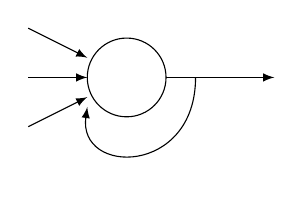
\begin{tikzpicture}[scale=2.5]
\draw (0, 0) circle (0.2cm);
\draw [-latex] (0.35, 0) .. controls (0.35, -0.5) and (-0.25, -0.5) .. (-0.2, -0.15);
\draw [-latex] (-0.5, 0.25) -- (-0.2, 0.1);
\draw [-latex] (-0.5, 0) -- (-0.2, 0);
\draw [-latex] (-0.5, -0.25) -- (-0.2, -0.1);
\draw [-latex] (0.2, 0) -- (0.75, 0);
\end{tikzpicture}
\caption{A recurrent neuron with a feedback loop}
\label{fig:rnn}
\end{figure}

\subsection{Long short-term memory (LSTM)}
Long short-term memory (LSTM) \cite{hochreiter97} is a major variant of recurrent neural networks. The training of regular RNNs is notoriously difficult because of the vanishing and exploding gradients problems. LSTM is designed to address these training issues. One of the main feature of LSTM is the constant error propagation in its memory unit. This is brought by the linear activation of the memory content at every timestep. But this also results in a complex structure as in shown Fig~\ref{fig:lstm}.

LSTM has a central memory unit ($\+c$) with three different types of multiplicative gating that controls the flow of information in the memory. The value of each gating at every time step is determined by a weighted sum of the current input ($\+x_t$), the current memory content ($\+c_t$), and the current output ($\+y_t$). A sigmoid function maps the weighted sum to a gating value between zero and one. The memory of each timestep is then updated by the forget gate ($\+f_t$) multiplying with the memory content from the previous time step, and the input gate ($\+i_t$) multiplying with the current input through a hyperbolic tangent (tanh) activation function. Lastly, the output of the neural network can be obtained by the output gate ($\+o_t$) multiplying with the current memory through another hyperbolic tangent activation. The equations of LSTM are summarized in Equation~\ref{eq:lstm}.

\begin{figure}
\centering
\begin{tikzpicture}[font=\small]

% Central memory unit
\draw (0,0) rectangle (1,3);
\draw (0.5,2.5) circle (0.3cm);
\draw (0.5,1.5) circle (0.3cm);
\draw (0.5,0.5) circle (0.3cm);

% Output gates
\draw (2,1.5) circle (0.2cm);
\draw (3,1.5) circle (0.1cm);
\draw (3,1.0) circle (0.2cm);

% Input gates
\draw (-1,1.5) circle (0.2cm);
\draw (-2,1.5) circle (0.1cm);
\draw (-2,1.0) circle (0.2cm);

% Forget gates
\draw (0.5,-0.5) circle (0.1cm);
\draw (0.5,-1) circle (0.2cm);

% Output connections
\draw [-latex](1,1.5) -- (1.8,1.5);
\draw [-latex](2.2,1.5) -- (2.9,1.5);
\draw [-latex](3.1,1.5) -- (4,1.5);
\draw [-latex](3,1.2) -- (3,1.4);

% Input connections
\draw [-latex](-3,1.5) -- (-2.1,1.5);
\draw [-latex](-1.9,1.5) -- (-1.2,1.5);
\draw [-latex](-0.8,1.5) -- (0,1.5);
\draw [-latex](-2,1.2) -- (-2,1.4);

% Forget connections
\draw [-latex](1.35,1.5) .. controls (1.4,-0.5) .. (0.6, -0.5);
\draw [latex-](-0.35,1.5) .. controls (-0.4,-0.5) .. (0.4, -0.5);
\draw [-latex](0.5,-0.8) -- (0.5,-0.6);

% Output gating inputs
\draw [-latex](2.7,0.4) -- (2.9,0.8);
\draw [-latex](3.0,0.4) -- (3.0,0.8);
\draw [-latex](3.3,0.4) -- (3.1,0.8);

% Input gating inputs
\draw [-latex](-2.3,0.4) -- (-2.1,0.8);
\draw [-latex](-2.0,0.4) -- (-2.0,0.8);
\draw [-latex](-1.7,0.4) -- (-1.9,0.8);

% Forget gating inputs
\draw [-latex](0.2,-1.6) -- (0.4,-1.2);
\draw [-latex](0.8,-1.6) -- (0.6,-1.2);

% Notations
\path (-3.3,1.5) node[draw=none] (X1) {$\+x_t$};
\path (-2.5,0.1) node[draw=none] (X2) {$\+x_t$};
\path (0.1,-1.9) node[draw=none] (X3) {$\+x_t$};
\path (2.5,0.1) node[draw=none] (X4) {$\+x_t$};
\path (4.2,1.5) node[draw=none] (Y1) {$\+y_t$};
\path (-1.1,0.1) node[draw=none] (Y2) {$\+y_{t-1}$};
\path (1.1,-1.9) node[draw=none] (Y3) {$\+y_{t-1}$};
\path (3.9,0.1) node[draw=none] (Y4) {$\+y_{t-1}$};
\path (0.5,1.5) node[draw=none] (C1) {$\+c_t$};
\path (-1.9,0.1) node[draw=none] (C2) {$\+c_{t-1}$};
\path (3.1,0.1) node[draw=none] (C3) {$\+c_t$};
\path (-1.5,1.0) node[draw=none] (I) {$\+i_t$};
\path (3.5,1.0) node[draw=none] (O) {$\+o_t$};
\path (1,-1) node[draw=none] (F) {$\+f_t$};

% Activation function
\draw (0.31,-1.1) .. controls (0.6,-1.1) and (0.4,-0.9) .. (0.69,-0.9);
\draw (-1.19,1.4) .. controls (-0.9,1.4) and (-1.1,1.6) .. (-0.81,1.6);
\draw (1.81,1.4) .. controls (2.1,1.4) and (1.9,1.6) .. (2.19,1.6);
\draw (-2.19,0.9) .. controls (-1.9,0.9) and (-2.1,1.1) .. (-1.81,1.1);
\draw (2.81,0.9) .. controls (3.1,0.9) and (2.9,1.1) .. (3.19,1.1);

\end{tikzpicture}
\caption{Long short-term memory}
\label{fig:lstm}
\end{figure}

\begin{equation}
\label{eq:lstm}
    \begin{array}{r c l}
\+i_t &=& \sigma(\+W_{ix} \+x_t + \+W_{iy} \+y_{t-1} + \+W_{ic} \+c_{t-1} + \+b_i)\\
\+f_t &=& \sigma(\+W_{fx} \+x_t + \+W_{fy} \+y_{t-1} + \+W_{fc} \+c_{t-1} + \+b_f)\\
\+z_t &=& \tanh(\+W_{cx} \+x_t + \+W_{cy} \+y_{t-1} + \+b_c)\\
\+c_t &=& \+f_t \odot \+c_{t-1} + \+i_t \odot \+z_t\\
\+o_t &=& \sigma(\+W_{ox} \+x_t + \+W_{oy} \+y_{t-1} + \+W_{oc} C_t + \+b_o)\\
\+y_t &=& \+o_t \odot \tanh(\+c_t)
    \end{array}
\end{equation}

Here, $\sigma$ denotes the sigmoid function, and $\odot$ denotes component-wise product. $\+x_t$ is a $D$ dimensional input vector at time $t$. $\+W_{ix}, \+W_{iy}, \+W_{ic}$ are $M \times D$ dimension weight matrices, which maps the input dimension to the memory dimension. Other weight matrices are of dimension $M \times M$. $\+y_t$ and $ \+c_t$ are output and memory content vector of dimension $M$ at time $t$. And $\+b_i, \+b_f, \+b_c, \+b_o$ are bias vectors of dimension $M$.

\subsection{Training of RNNs}
The training of RNNs is typically achieved by backpropagation through time (BPTT) \cite{mozer95}. The idea is to imagine the recurrent network as a chain of feedforward network by unfolding the recurrent connections through time. The error derivatives can then be evaluated as in normal feedforward networks. In the end, the errors to weight connections are summed up through time.

\begin{equation}
\dfrac{\del E}{\del \+W} = \sum_t{\left(\dfrac{\del E}{\del \+W}\right)_t}
\end{equation}

\begin{figure}  
\centering
\begin{tikzpicture}
\draw (1.35,1.5) .. controls (1.4,-0.5) .. (0.5, -0.5);
\draw [latex-](-0.35,1.5) .. controls (-0.4,-0.5) .. (0.5, -0.5);
%\draw [-latex](1,1.5) .. controls (3, -1) and (-2, -1) .. (0,1.5);
\foreach \x in  {0, 7, 9, 13}
{
	\draw (\x,0) rectangle (\x+1,3);
	\draw (\x+0.5,2.5) circle (0.3cm);
	\draw (\x+0.5,1.5) circle (0.3cm);
	\draw (\x+0.5,0.5) circle (0.3cm);
	\draw [-latex](\x-1,1.5) -- (\x,1.5);
	\draw [-latex](\x+1,1.5) -- (\x+2,1.5);
}
\foreach \x in  {7, 9, 13}
{
	\draw [latex-](\x-1,1.25) -- (\x,1.25);
	\draw [latex-](\x+1,1.25) -- (\x+2,1.25);
}
\path (1, -2) node[draw=none] (left_title) {Recurrent neural network};
\path (11,-2) node[draw=none] (right_title) {Unfolded through time};
\path (0.5,-1) node[draw=none] (tA) {$t=0...T-1$};
\path (7.5,-1) node[draw=none] (t0) {$t=0$};
\path (9.5,-1) node[draw=none] (t1) {$t=1$};
\path (13.5,-1) node[draw=none] (tT1) {$t=T-1$};
\path (7.5,-0.5) node[draw=none] (t0) {$(\del E / \del \+W)_0$};
\path (9.5,-0.5) node[draw=none] (t1) {$(\del E / \del \+W)_1$};
\path (13.5,-0.5) node[draw=none] (tT1) {$(\del E / \del \+W)_{T-1}$};
\path (-0.5,1.75) node[draw=none] (Xleft) {$\+x$};
\path (1.5,1.75) node[draw=none] (Yleft) {$\+y$};
\path (6.5,1.75) node[draw=none] (Xleft) {$\+x$};
\path (14.5,1.75) node[draw=none] (Yleft) {$\+y$};
\path (6.5,0.7) node[draw=none] (Xleft) {$\dfrac{\del E}{\del \+x}$};
\path (14.5,0.7) node[draw=none] (Yleft) {$\dfrac{\del E}{\del \+y}$};
\draw [dotted] (11,1.5) -- (12,1.5);
\end{tikzpicture}
\caption{Back-propagation through time}
\label{fig:bptt}
\end{figure}

More RNN training techniques can be found in Appendix \ref{train_tech}.

\section {Word embedding}
In the previous sections, we have covered some neural network basics and popular configurations. In the following sections, we will introduce some recent applications in the field of natural language processing and question answering using word embeddings and recurrent neural networks.

A short definition for word embedding is a dictionary which assigns each vocabulary a high dimensional vector that captures semantic similarity. Typical English vocabulary size in NLP applications are between 10,000 and 100,000, and following the Zipf's law\cite{zipf49}, most of the vocabularies are rare words. In a typical n-gram analysis, our computational and storage resource quickly run out because of the sparsity of word combinations. To fight against this curse of dimensionality, one would like to share knowledge between similar words without redundant training examples for each word. For example in a language modelling task, if we have seen the sentence ``the cat is walking in the bedroom'', then the other sentence ``the dog was running in a room'' should also be assigned with higher probability \cite{bengio03}. While traditional non-parametric n-gram models fail to capture the associativity of similar words, neural networks have the ability to approximate the probability distribution over a continuous hyperspace. But to enable this task, we need to convert every word into its vector representation. We can first randomly initialize the word embedding matrix as the first layer of a neural network, and then train the network to predict the next word given a sequence of previous words. In the end, the first layer can be then used as a fine-tuned word embedding. The trained embedding vectors are distributed representation of words that preserve semantic similarity. Earlier word embeddings are mostly trained from neural language models, until recently researchers found that language modelling is not necessary to obtain a good word embedding.

\subsection{Skip-gram embedding model}
The skip-gram model \cite{mikolov13} is a very successful word embedding model. In the paper, the authors used two methods to train word vectors: the continuous bag of words (CBOW) and the skip gram model. The former aims to predict the missing word given a bag of context words, and the latter aims to predict the context surrounding a given single word. The model is streamlined to one single linear mapping which significantly shortens the training time down to a few minutes on a standard computer, as opposed to a few weeks for neural language models. It is also astonishing to see algebraic operators can be directly applied on word vectors, and can preserve the intended meaning. For example, ``king'' + 	``woman'' - ``man'' $\sim$ ``queen'' \cite{mikolov13}. The software package released with the paper is called ``word2vec.'' A lot of subsequent research directly uses this software to train general purpose or problem specific word embeddings.

\section{Jointly learn image and word}
Human beings are capable of associating objects of their different forms. For example, when people see a text ``pink pig'', they are likely to imagine a picture of a pink pig in their head. Likely, when people see blue sky in their eyes, they are likely to have some word-level mental activity. It is an intriguing question to ask if we can engineer a ``visual-semantic joint embedding,'' an abstract vector space in which the word ``sky'' and a picture of sky has very small distance. It is very tempting to build such an embedding on top of the existing convolutional neural networks and word embeddings. In the work ``Deep Visual-Semantic Embedding Model'' (DeViSE) \cite{frome13}, researchers used model proposed earlier \cite{weston10} but replaced the image feature extractors with the last hidden layer convolutional net \cite{krizhevsky12} (just before the softmax layer). The image representation is then mapped to the word embedding space \cite{mikolov13} with a linear transformation. The model is trained to correctly classify images, and the joint embedding outperforms the standard convolutional neural net by a large margin on a test set with a large number of unseen classes. The reason is that even though the exact images of the classes are unseen, the class names have already had their word similarity captured in the word embedding space, and thus beat the simple fully connected softmax layer in standard convolutional neural networks. Not only does joint embedding improves the result for image object recognition tasks, it also encourages better cooperation of visual and semantic knowledge. The work by \cite{kiros14b} proposed models that generate descriptions based on an image input using visual semantic embeddings, and the generated sentences have much better plausibility and accuracy compared to earlier results \cite{kulkarni11,mitchell12}. In their work, they used LSTM introduced earlier as part of the encoder of training descriptions as well as the decoder of generated descriptions. These recent works have shown us very strong feasibility to jointly learn image and text in a joint embedding space.

\section{Image-based question answering}
The following sections will focus on the background of question-answering and recent research specifically related to image-based question answering. Traditional QA builds entity relationships within a large text collection, or a corpus, using natural language processing (NLP) techniques. Large-scale question answering has a long history, mostly initiated via the Text Retrieval Conference (TREC). Despite some eminent successes in building such systems, such as \cite{lewis12}, building a knowledge graph requires a great amount of engineering and is heavily dependent on the knowledge base or the search engine, and is also hard to generalize to unseen entities. There have been ongoing efforts of using embedding-based model and recurrent neural networks on question-answering tasks. \cite{weston14} showed that their memory-based recurrent neural network can perfectly answer questions that involve long time dependency in a paragraph.

Image-based question answering has its own differences compare to text-based question answering:
First, the question is centered on the image. Therefore, the model needs to acquire both visual and semantic knowledge.
Second, unlike traditional question answering where the training data contains almost the exact answer with certain predicates revealing its relation with the question, here the training data provides no direct information to the answer, which is solely contained the unseen test image. However, the training data provides very strong clue of what catagories of answers are expected. For example, the model should be able to conclude from the training data that ``chair'' is a more probable answer than ``window'' for a question like ``What is around the table?''  These differences actually make the problem unique from traditional QA tasks.

\subsection{DAQUAR dataset}
\label{background_daquar}
In 2014, Malinowski et al. released a dataset with images and question-answer pairs. It is called DAtaset for QUestion Answering on Real-world images (DAQUAR) \cite{malinowski14a}. All images are from the NYU depth v2 dataset \cite{silberman12}, and are taken from indoor scenes. Human segmentations, image depth values, and object labellings are available in the dataset. The QA pairs were created by human crowdsourcing. The original train-test split ratio is about 3800:3300. The QA data has two sets of configuration: the 37-class and the 894-class dataset, differed by the number of object classes appearing in the questions. There are mainly three types of questions in this dataset:
\begin{enumerate}
	\item Object type
	\item Object colour
	\item Number of objects
\end{enumerate}
Qualitatively speaking, a large proportion of the questions are very hard to answer. Figure~\ref{fig:difficult} summarizes the sources of difficulties. Since DAQUAR is the only publicly available image-based QA dataset, it is one of our benchmarks to evaluate our models.

\begin{figure}
    \centering
    \footnotesize
    \begin{subfigure}[t]{0.3\textwidth}
            \includegraphics[width=\textwidth]{red.jpg}
            Q7: what colour is the ornamental plant in fornt of the fan coil but not close to sofa ? -red
            \caption{Hard to locate the object}
    \end{subfigure}%
    \quad
    \begin{subfigure}[t]{0.3\textwidth}
            \includegraphics[width=\textwidth]{black.jpg}
            Q20: how many black objects are on the desk ? -three
            \caption{Counting ambiguity, could be three to five}
    \end{subfigure}
    \quad
    \begin{subfigure}[t]{0.3\textwidth}
            \includegraphics[width=\textwidth]{blind.jpg}
            Q1129: what is behind the tap ? -blinds
            \caption{Object ambiguity, could be a window or blinds}
    \end{subfigure}
    \quad
    \begin{subfigure}[t]{0.3\textwidth}
            \includegraphics[width=\textwidth]{sink.jpg}
            Q5: what is under the white cabinet on the right side of the oven and and on the left side of the fridge ? -sink
            \caption{Lengthy description of spatial relations}
    \end{subfigure}
    \quad
    \begin{subfigure}[t]{0.3\textwidth}
            \includegraphics[width=\textwidth]{brown.jpg}
            Q1423: what is the colour of the furniture ? -brown
            \caption{Colour ambiguity due to dim lighting}
    \end{subfigure}
    \quad
    \begin{subfigure}[t]{0.3\textwidth}
            \includegraphics[width=\textwidth]{paper.jpg}
            Q1467: what is on the night stand ? -paper
            \caption{Object is too small}
    \end{subfigure}
    \caption{Various types of difficult questions in the DAQUAR dataset}
	\label{fig:difficult}
\end{figure}

\subsection{Previous attempt}
Together with the release of the DAQUAR dataset, \cite{malinowski14b} presented an approach which combines semantic parsing and image segmentation. In the natural language part of their work, they used a semantic parser \cite{liang13} to convert sentences into latent logical forms. The parser is specially designed for QA tasks, and can be trained well where the true dependency tree is missing from the training data. In the image part, they evaluated different latent logical forms of the question with multiple segmentation. They obtained the multiple segmentations of the image by sampling the uncertainty of the segmentation algorithm. Their model is based on a Bayesian formulation that every logical form and image segmentation has certain probability. To make the inference step of their algorithm scalable, they chose to sample from the nearest neighbours in the training set according to the similarity of the semantic parsing.

While their model seems to handle a number of spatial relations, their predefined set of possible predicates constrains the question form and the environment. Moreover, the quality of answers also depends on the accuracy of the automatic image segmentation algorithm. Lastly, inferring all possible predicates between every pair of objects does not scale to larger dataset. The embedding space models introduced earlier have significant differences with their approach, and we hope that our embedding space model will outperform their model in terms of answer accuracy and similarity.